% Informe final del Proyecto 2 (Entregable 2).
% Se compila con: docker build -t pvlt-informe docs/informe
%                 docker run --rm -v "${PWD}:/work" -w /work/docs/informe pvlt-informe latexmk -pdf informe.tex
\documentclass[11pt,letterpaper]{article}

\usepackage[T1]{fontenc}
\usepackage[utf8]{inputenc}
\usepackage[spanish,es-noshorthands,es-tabla]{babel}
\usepackage{mathpazo}
\usepackage{lmodern}
\renewcommand{\rmdefault}{ppl}
\renewcommand{\ttdefault}{lmtt}
\usepackage{microtype}
\usepackage[margin=2.1cm]{geometry}
\usepackage{amsmath,amssymb}
\usepackage{booktabs,tabularx,array}
\usepackage{graphicx}
\usepackage{caption}
\usepackage{subcaption}
\usepackage[dvipsnames]{xcolor}
\usepackage{tikz}
\usetikzlibrary{positioning,arrows.meta,decorations.pathreplacing,calc,fit,backgrounds}
\usepackage{enumitem}
\usepackage{titlesec}
\usepackage{fancyhdr}
\usepackage[hidelinks]{hyperref}

\definecolor{tinta}{HTML}{2B3A55}
\definecolor{gris}{HTML}{8A8F98}
\definecolor{azulc}{HTML}{E3ECF8}
\definecolor{azul}{HTML}{3A6FB0}
\definecolor{rojoc}{HTML}{FBE3E3}
\definecolor{rojo}{HTML}{C0392B}
\definecolor{verdec}{HTML}{E2F3E5}
\definecolor{verde}{HTML}{3C8D4C}
\definecolor{amar}{HTML}{FFF3D6}
\definecolor{naranja}{HTML}{D9902B}

\titleformat{\section}{\large\bfseries\color{tinta}}{\thesection.}{0.5em}{}
\titleformat{\subsection}{\normalsize\bfseries\color{tinta}}{\thesubsection}{0.5em}{}
\titlespacing*{\section}{0pt}{1.2ex plus .3ex}{0.6ex}
\titlespacing*{\subsection}{0pt}{1ex plus .3ex}{0.4ex}
\captionsetup{font=small,labelfont=bf,labelsep=colon}
\setlist{itemsep=1pt,topsep=3pt,leftmargin=1.3em}
\setlength{\parskip}{0.45ex}
\renewcommand{\arraystretch}{1.12}

\pagestyle{fancy}
\fancyhf{}
\fancyfoot[L]{\small\thepage}
\fancyfoot[R]{\small\color{gris}Informe final · Proyecto 2}
\renewcommand{\headrulewidth}{0pt}

\newcommand{\code}[1]{\texttt{#1}}
\newcommand{\pvlt}{\code{pvlt}}

\begin{document}

\begin{center}
{\LARGE\bfseries\color{tinta} Gestor local de contraseñas con Argon2id y AEAD}\\[3pt]
{\large Proyecto 2 · Entregable 2: implementación, pruebas y experimentos}\\[2pt]
{\small Criptografía Aplicada, Universidad del Norte · Docente: Ricardo Luis Villanueva-Polanco}\\[2pt]
{\small Integrantes: Carlos Ruidiaz · Juan Bolivar · Juan Rojas · Claudia Elias}\\[2pt]
{\small Repositorio: \url{https://github.com/CarlosRuidiaz/Gestor-local-de-contrase-as}}
\end{center}
\vspace{-1ex}
{\color{gris}\rule{\linewidth}{0.4pt}}

\begin{abstract}
\noindent
Se implementó \pvlt, un gestor de contraseñas de un solo usuario que funciona por completo en el equipo, con interfaz web local y un CLI mínimo. La contraseña maestra deriva con Argon2id una clave que envuelve una clave de datos aleatoria, renovada en cada guardado, que cifra el contenido con ChaCha20-Poly1305. La cabecera completa del archivo es dato asociado de ambos cifrados. El producto cumple el diseño del Entregable 1 sin cambios en el formato ni en el protocolo, y lo concreta en los puntos que el diseño dejaba abiertos. Una suite de 673 pruebas automatizadas cubre los trece casos del plan, incluidos manipulación byte a byte, caídas tras cada paso del guardado y ataques contra el servidor local. Los experimentos fijan la configuración final de Argon2id en 256 MiB, 3 pasadas y 4 carriles, que desbloquea en 0,42 s en el equipo de referencia y obliga a un atacante a gastar unas 4\,100 horas de núcleo para recorrer un diccionario del tamaño de RockYou.
\end{abstract}

\section{Introducción y alcance}

El enunciado del Proyecto 2 pide un gestor local que cree, desbloquee y bloquee una bóveda de 1 a 500 credenciales, con generador, bloqueo por inactividad, cambio de contraseña maestra, exportación e importación cifradas y recuperación segura ante fallos durante el guardado~\cite{enunciado}. Exige además Argon2id v1.3 con sal aleatoria, un AEAD estándar de una biblioteca mantenida, nonces únicos, metadatos autenticados, un formato versionado y que ningún secreto aparezca en logs, temporales ni argumentos del proceso.

El Entregable 1 propuso el diseño. Este informe describe lo que se construyó a partir de él, cómo se verificó y qué se midió. La sección~\ref{sec:modelo} recuerda el modelo de adversario. Las secciones~\ref{sec:protocolo} y~\ref{sec:arquitectura} presentan el protocolo y la arquitectura implementados. La sección~\ref{sec:desviaciones} enumera las desviaciones y concreciones respecto al diseño. Las secciones~\ref{sec:pruebas} y~\ref{sec:experimentos} reportan las pruebas y los experimentos, y la sección~\ref{sec:limitaciones} discute los límites de seguridad que quedan.

El producto es un repositorio ejecutable con Docker. Un \code{docker compose up} arranca la interfaz web, \code{docker compose run -{}-rm app pytest} ejecuta la suite completa y \code{python -m scripts.demo} recorre cada escenario de la demostración exigida con datos sintéticos. El README del repositorio detalla la instalación desde cero y el guion de demostración. La tabla~\ref{tab:enunciado} indica dónde se resuelve cada decisión de diseño que el enunciado deja al equipo.

\begin{table}[h]
\centering\small
\caption{Decisiones que el enunciado pide resolver y dónde se tratan.}
\label{tab:enunciado}
\begin{tabularx}{\linewidth}{@{}>{\raggedright\arraybackslash}X>{\raggedright\arraybackslash}p{0.42\linewidth}@{}}
\toprule
Decisión del enunciado & Dónde y con qué evidencia \\
\midrule
Parámetros de Argon2id para el equipo de ejecución & §\ref{sec:justificacion} y E1 (§\ref{sec:experimentos}), \code{bench.calibrate} \\
Estructura pública y cifrada del archivo & §3.2, figura~\ref{fig:formato}, T4 y T5 \\
Unicidad de nonces tras cierres inesperados o reintentos & §3.4 y T6 \\
Cambiar la contraseña maestra y distinguir contraseña incorrecta de archivo dañado & §3.3, §3.5, §\ref{sec:justificacion}, T2 y T4 \\
Guardado atómico que no sustituye una bóveda válida por una incompleta & §\ref{sec:arquitectura} y T7 \\
Ataques que una aplicación local no puede evitar & §\ref{sec:modelo} y §\ref{sec:limitaciones} \\
\bottomrule
\end{tabularx}
\end{table}

\section{Escenario y modelo de adversario}\label{sec:modelo}

El usuario ejecuta \pvlt{} en su propio equipo. El servidor escucha solo en la interfaz local, descifra la bóveda en su memoria tras recibir la contraseña maestra por un POST local y la vuelve a cifrar en cada cambio. En disco solo existen la bóveda, su respaldo y, durante un guardado, un temporal, todos cifrados con el mismo formato.

\begin{table}[h]
\centering\small
\caption{Adversarios del modelo, propiedades que se le oponen y pruebas que las verifican.}
\label{tab:adversarios}
\begin{tabularx}{\linewidth}{@{}l>{\raggedright\arraybackslash}X>{\raggedright\arraybackslash}Xl@{}}
\toprule
Id & Adversario y capacidad & Propiedad y mecanismo & Evidencia \\
\midrule
A1 & Lector fuera de línea que copia el archivo y prueba contraseñas con hardware paralelo & P1 confidencialidad (AEAD, relleno a 4 KiB) y P2 costo por intento (Argon2id, sal de 128 bits) & T3, T8, E1 \\
A2 & Manipulador que altera, trunca o reemplaza el archivo & P3 integridad (cabecera como dato asociado) y P7 parámetros acotados & T4, T5 \\
A3 & Fallo no malicioso que interrumpe un guardado o daña bytes & P4 nonces únicos (DEK nueva por guardado) y P5 guardado atómico & T6, T7 \\
A4 & Usuario local sin privilegios que lee argumentos, entorno y archivos laxos y se conecta a puertos locales & P6 ningún secreto fuera de memoria y P8 servidor usable solo por el usuario & T9, T12, T13 \\
A5 & Página web maliciosa que intenta CSRF, DNS rebinding o incrustar la aplicación & P8 (token de arranque, cookie \code{SameSite=Strict}, CSRF, Host y Origin, CSP) & T13 \\
\bottomrule
\end{tabularx}
\end{table}

Quedan fuera del modelo, como en el Entregable 1, el malware, los keyloggers, las extensiones maliciosas, los volcados de memoria con la bóveda abierta, las contraseñas maestras muy débiles, la observación física y el retroceso a una copia antigua válida, que solo se advierte.

\section{Protocolo criptográfico implementado}\label{sec:protocolo}

\subsection{Jerarquía de claves}

Con $\mathrm{Hdr}$ los 59 bytes de la cabecera tal como se escriben en disco y $P$ el contenido, cada guardado calcula
\begin{align*}
\mathit{KEK} &= \mathrm{Argon2id}_{v1.3}(pw,\ salt,\ m,\ t,\ p,\ 32)\\
W &= \mathrm{ChaCha20\text{-}Poly1305}(\mathit{KEK}).\mathrm{Enc}(N_w,\ \mathit{DEK},\ \texttt{"PVLT/v1/wrap"} \,\|\, \mathrm{Hdr})\\
C &= \mathrm{ChaCha20\text{-}Poly1305}(\mathit{DEK}).\mathrm{Enc}(N_d,\ \mathrm{pad}(P),\ \texttt{"PVLT/v1/data"} \,\|\, \mathrm{Hdr} \,\|\, W)
\end{align*}
La KEK de la bóveda solo se deriva al crear, al desbloquear y al cambiar la contraseña, y vive en memoria durante la sesión. Exportar e importar derivan además una KEK propia con la contraseña de exportación, que se borra en cuanto se usa. Cada guardado genera con \code{secrets} una DEK de 32 bytes y nonces $N_w$ y $N_d$ de 12 bytes nuevos, de modo que guardar no repite Argon2id (figura~\ref{fig:claves}). Las etiquetas de dominio impiden que un bloque de envoltura se acepte como contenido, y la inclusión de $W$ en el dato asociado de $C$ ata el contenido a su DEK envuelta. Así el AEAD autentica tanto los datos como todos los metadatos críticos, que es la propiedad de integridad de textos cifrados que da a un esquema AEAD su seguridad frente a manipulación~\cite[§9.5]{boneh}.

\begin{figure}[h]
\centering
\begin{tikzpicture}[
  font=\small,
  caja/.style={draw=#1, rounded corners=2pt, align=center, inner sep=4pt, minimum height=9mm, minimum width=36mm},
  flecha/.style={-{Stealth[length=2mm]}, gris, thick},
  ad/.style={-{Stealth[length=2mm]}, gris, dashed},
  rot/.style={font=\scriptsize, text=gris}]
\node[caja=rojo, fill=rojoc] (pw) at (0,0) {\textbf{Contraseña maestra}\\[-1pt]{\scriptsize POST local, sin eco}};
\node[caja=gris, fill=white] (argon) at (5,0) {\textbf{Argon2id v1.3}\\[-1pt]{\scriptsize sal 16 B, $m$, $t$, $p$}};
\node[caja=azul, fill=azulc] (kek) at (10,0) {\textbf{KEK, 32 B}\\[-1pt]{\scriptsize solo en memoria}};
\node[caja=azul, fill=azulc] (dek) at (2.5,-1.9) {\textbf{DEK, 32 B}\\[-1pt]{\scriptsize nueva en cada guardado}};
\node[caja=gris, fill=white, minimum width=44mm] (c) at (2.5,-4.0) {\textbf{Contenido $C$}\\[-1pt]{\scriptsize ChaCha20-Poly1305 con la DEK}};
\node[caja=gris, fill=white, minimum width=44mm] (w) at (8.5,-4.0) {\textbf{DEK envuelta $W$}\\[-1pt]{\scriptsize ChaCha20-Poly1305 con la KEK}};
\node[caja=naranja, fill=amar, minimum width=104mm] (hdr) at (5.5,-5.8) {\textbf{Cabecera pública Hdr}\\[-1pt]{\scriptsize versión, algoritmos, parámetros, sal, id, generación}};
\begin{scope}[on background layer]
\node[draw=gris!60, fill=gray!6, rounded corners=3pt, fit=(c)(w)(hdr), inner sep=7pt] (disco) {};
\end{scope}
\node[rot, anchor=north east] at (disco.south east) {archivo en disco};
\draw[flecha] (pw) -- (argon);
\draw[flecha] (argon) -- (kek);
\draw[flecha] (kek.south -| 10,0) -- node[rot, right]{envuelve} (w.north -| 10,0);
\draw[flecha] (dek.east) -| node[rot, pos=0.25, above]{se envuelve} (w.north -| 7.2,0);
\draw[flecha] (dek) -- node[rot, right]{cifra} (c);
\draw[ad] (hdr.north -| c) -- node[rot, right]{AD} (c.south);
\draw[ad] (hdr.north -| w) -- node[rot, right]{AD} (w.south);
\draw[ad] (w) -- node[rot, above]{AD} (c);
\end{tikzpicture}
\caption{Jerarquía de claves. La contraseña solo protege la DEK. La cabecera es dato asociado de ambos cifrados y $W$ también lo es de $C$.}
\label{fig:claves}
\end{figure}

\subsection{Formato binario v1}

El archivo es binario, con campos de longitud fija y enteros big-endian, de modo que cada bóveda tiene una única serialización (figura~\ref{fig:formato}). La cabecera contiene \code{magic} \code{"PVLT"}, \code{format\_version}, \code{purpose} (\code{0x01} bóveda, \code{0x02} exportación), los identificadores de KDF y AEAD, la versión de Argon2 (\code{0x13}), $m$, $t$, $p$, la sal, un \code{vault\_id} aleatorio y un contador \code{generation}. Siguen $N_w$, $W$, $N_d$, la longitud de $C$, el propio $C$ y un SHA-256 de todo lo anterior. La parte fija ocupa 135 bytes, y con el resumen y la etiqueta de $C$ el exceso sobre el contenido rellenado es de 183 bytes.

\begin{figure}[h]
\centering
\begin{tikzpicture}[font=\scriptsize, campo/.style={draw=gris, minimum height=8mm, align=center, inner sep=1pt}]
\node[campo, fill=amar, minimum width=24mm] (h) {\textbf{Hdr}\\59 B};
\node[campo, minimum width=12mm, right=0pt of h] (nw) {$N_w$\\12 B};
\node[campo, fill=azulc, minimum width=16mm, right=0pt of nw] (w) {$W$\\48 B};
\node[campo, minimum width=12mm, right=0pt of w] (nd) {$N_d$\\12 B};
\node[campo, minimum width=12mm, right=0pt of nd] (l) {\code{len\_C}\\4 B};
\node[campo, fill=azulc, minimum width=44mm, right=0pt of l] (c) {$C$\\$4096k + 16$ B};
\node[campo, fill=gray!10, minimum width=16mm, right=0pt of c] (d) {\code{digest}\\32 B};
\draw[decorate, decoration={brace, amplitude=4pt, mirror}, gris] ([yshift=-1mm]h.south west) -- node[below=4pt]{AD de $W$ (etiqueta \emph{wrap})} ([yshift=-1mm]h.south east);
\draw[decorate, decoration={brace, amplitude=4pt, mirror}, gris] ([yshift=-7mm]h.south west) -- node[below=4pt]{AD de $C$ (etiqueta \emph{data})} ([yshift=-7mm]w.south east);
\draw[decorate, decoration={brace, amplitude=4pt}, gris] ([yshift=1mm]h.north west) -- node[above=4pt]{cubierto por el SHA-256 final, que solo detecta errores accidentales} ([yshift=1mm]c.north east);
\end{tikzpicture}
\caption{Estructura del archivo y cobertura de los datos asociados.}
\label{fig:formato}
\end{figure}

El contenido $P$ es JSON UTF-8 canónico, con claves ordenadas y sin espacios, que lleva la versión de esquema, la lista de entradas (identificador UUID v4, sitio, usuario, contraseña, notas y fechas en UTC) y los ajustes. Se rellena con \code{0x80} seguido de ceros hasta un múltiplo de 4096 bytes, así que el tamaño del archivo solo revela un rango del número de entradas. \code{format\_version} y \code{schema} versionan por separado la estructura binaria y el contenido, y cualquier versión desconocida se rechaza.

\subsection{Desbloqueo en cuatro comprobaciones}

Abrir un archivo aplica cuatro comprobaciones en orden, cada una con su excepción y su mensaje, y ninguna escribe en disco ni crea una bóveda vacía.
\begin{enumerate}
\item \textbf{Formato.} Longitud total exacta, \code{magic}, versión, propósito, identificadores de algoritmo, versión de Argon2, \code{len\_C} coherente y parámetros dentro de límites ($m \le 4$ GiB, $1 \le t, p \le 16$, $m \ge 8p$). Falla con «Formato no reconocido». Los límites se validan \emph{antes} de ejecutar Argon2id, para que una cabecera manipulada no agote la memoria.
\item \textbf{Resumen.} El SHA-256, comparado en tiempo constante. Falla con «Archivo dañado» y la interfaz ofrece el respaldo.
\item \textbf{Abrir $W$} con la KEK. Falla con «Contraseña incorrecta».
\item \textbf{Abrir $C$} con la DEK, quitar el relleno y validar el JSON de forma estricta. Falla con «Contenido manipulado».
\end{enumerate}
Un atacante puede recalcular el resumen, así que la aceptación depende siempre de las comprobaciones 3 y 4. Una alteración de la sal, de cualquier otro campo de la cabecera que siga dentro de los límites, de $N_w$ o de $W$ hace fallar la comprobación 3 y se informa como contraseña incorrecta, porque sin la clave ambos casos son indistinguibles. Es la limitación que el Entregable 1 ya declaraba.

\subsection{Unicidad de nonces sin contador}

Cada DEK cifra un único mensaje, así que bajo ella la unicidad del nonce es estructural. Bajo la KEK cada guardado usa un nonce aleatorio de 96 bits, y tras $q$ guardados la probabilidad de colisión es a lo sumo $q^2/2^{97}$. Se adopta de forma conservadora la cota de $2^{32}$ cifrados por clave que SP~800-38D fija para nonces aleatorios~\cite{sp80038d}. Mil guardados diarios durante diez años suman unos $2^{22}$. La KEK además cambia con cada cambio de contraseña. Un guardado interrumpido y reintentado toma valores nuevos, de modo que una caída nunca provoca reutilización. Se descartó un contador persistente como el número de secuencia de TLS~1.3~\cite{protocols} porque exige escribirlo de forma atómica antes de cada cifrado, y un error en ese orden llevaría justo a la reutilización que se quiere evitar.

\subsection{Operaciones sobre la bóveda}

\textbf{Cambiar la contraseña maestra} verifica la actual derivando con la sal vigente y abriendo $W$ del archivo en disco, genera sal nueva, deriva otra KEK y guarda. Después reescribe también el respaldo, para que ningún archivo siga abriéndose con la contraseña anterior. \textbf{Exportar} usa el mismo formato con \code{purpose} \code{0x02}, contraseña, sal, KEK y \code{vault\_id} propios. \textbf{Importar} aplica las mismas cuatro comprobaciones exigiendo ese propósito, muestra una vista previa y, si coincide el UUID o el par sitio y usuario, deja elegir entre omitir, sustituir o conservar ambas. \textbf{El generador} usa solo \code{secrets} con muestreo por rechazo: genera candidatas uniformes sobre la unión de las clases elegidas y descarta las que no contienen todas. El resultado es uniforme sobre las contraseñas válidas, y la entropía mostrada, longitud por $\log_2$ del alfabeto, es una cota superior que excede la real en unos 0,15 bits con la configuración por defecto.

\subsection{Por qué estas elecciones y no otras}\label{sec:justificacion}

\textbf{Función de derivación.} Un gestor local enfrenta el peor caso de los ataques a contraseñas. Quien copia el archivo prueba candidatas fuera de línea, sin que nada limite los intentos, con un costo del orden de $|D|$ sobre un diccionario $D$~\cite[§18.4.4]{boneh}~\cite{protocols}. La única defensa es encarecer cada intento, y la tabla~\ref{tab:alternativas} resume las opciones según~\cite[§18.4]{boneh} y~\cite[§1]{rfc9106}. La sal de 128 bits anula las tablas precalculadas pero no el diccionario directo. Se descartó además una sal secreta (\emph{pepper}), porque en un gestor local no tendría dónde guardarse aparte del propio archivo.

\begin{table}[h]
\centering\small
\caption{Alternativas consideradas para la derivación de clave y el cifrado autenticado.}
\label{tab:alternativas}
\begin{tabularx}{\linewidth}{@{}l>{\raggedright\arraybackslash}X>{\raggedright\arraybackslash}X@{}}
\toprule
Opción & Ventaja & Por qué se eligió o se descartó \\
\midrule
PBKDF2 & Estándar y disponible en todas partes & Itera una PRF que ocupa poca área de chip, así que se paraleliza barato en GPU o ASIC. Descartada \\
scrypt & Exige memoria, el recurso escaso del hardware paralelo & Sus accesos dependen de la contraseña y filtran por canal lateral de caché. Descartada \\
\textbf{Argon2id} & Memoria configurable, accesos independientes de los datos en la primera mitad de la primera pasada y dependientes en el resto & Variante recomendada por RFC~9106~\cite{rfc9106}. \textbf{Elegida} \\
\midrule
AES-256-GCM & Estándar NIST, muy rápido con instrucciones AES-NI & Sin AES-NI las implementaciones en software pueden filtrar por tiempo. El campo \code{aead\_id} permitiría añadirlo en otra versión del formato \\
\textbf{ChaCha20-Poly1305} & RFC~8439~\cite{rfc8439}, de tiempo constante en software en cualquier procesador & Mismo nonce de 96 bits que GCM, suficiente con una DEK por guardado. \textbf{Elegido} \\
XChaCha20-Poly1305 & Nonce de 192 bits, aleatorio sin límite práctico & No es RFC ni está en \code{cryptography}. Descartado \\
\bottomrule
\end{tabularx}
\end{table}

\textbf{Parámetros de Argon2id.} RFC~9106 §4 recomienda dos configuraciones, una de 2 GiB con 1 pasada y otra de 64 MiB con 3 pasadas, ambas con 4 carriles. Son C y A, y B es una intermedia de 256 MiB. Se prioriza la memoria sobre las pasadas porque la memoria es lo que limita cuántos intentos corre a la vez un atacante con hardware paralelo. El equilibrio entre la espera del usuario y la resistencia se fijó con una regla explícita: la configuración de mayor memoria cuyo desbloqueo no supere 1 s en el equipo que ejecuta \pvlt. La sección~\ref{sec:experimentos} la aplica al equipo de referencia, y el script \code{bench.calibrate} la aplica a cualquier otro.

\textbf{Distinguir una contraseña incorrecta de un archivo dañado.} El archivo termina en un SHA-256 sin clave y no en un MAC. Un MAC necesitaría una clave derivada de la contraseña, así que no permitiría separar un fallo de disco de una contraseña equivocada sin antes ejecutar Argon2id. El resumen sin clave detecta los errores accidentales y permite ofrecer el respaldo, mientras la integridad frente a un atacante queda a cargo de las etiquetas AEAD, que sí dependen de la clave.

\textbf{Biblioteca.} Se usa solo \code{cryptography} (pyca). PyNaCl fija el paralelismo de Argon2id en 1, y \code{argon2-cffi} añadiría una segunda dependencia criptográfica y no permite derivar en un búfer propio. \code{cryptography} ofrece las dos primitivas, acepta el secreto y el dato asociado que exigen los vectores de RFC~9106 y deriva directamente en un \code{bytearray} que luego se sobrescribe con ceros.

\section{Arquitectura e implementación}\label{sec:arquitectura}

El código está en Python 3.12 y usa una sola biblioteca criptográfica, \code{cryptography} 50.0.2 sobre OpenSSL 4.0.3, que ofrece Argon2id y ChaCha20-Poly1305~\cite{pyca}. Se divide en cuatro capas con dependencias en un solo sentido (figura~\ref{fig:capas}), y una prueba de humo verifica que ninguna capa importa a otra prohibida.

\begin{figure}[h]
\centering
\begin{tikzpicture}[font=\small, node distance=5mm and 9mm,
  caja/.style={draw=gris, fill=white, rounded corners=2pt, align=center, inner sep=3pt, minimum height=11mm, minimum width=30mm},
  flecha/.style={-{Stealth[length=2mm]}, gris, thick}]
\node[caja, fill=gray!8] (nav) {\textbf{Navegador}\\{\scriptsize HTML, CSS y JS propios}};
\node[caja, right=of nav] (web) {\textbf{web/}\\{\scriptsize FastAPI local,}\\[-2pt]{\scriptsize seguridad HTTP}};
\node[caja, draw=azul, fill=azulc, right=of web] (vault) {\textbf{vault/}\\{\scriptsize sesión y entradas,}\\[-2pt]{\scriptsize única capa con la KEK}};
\node[caja, above right=-2mm and 9mm of vault] (crypto) {\textbf{crypto/}\\{\scriptsize funciones puras,}\\[-2pt]{\scriptsize sin disco}};
\node[caja, below right=-2mm and 9mm of vault] (storage) {\textbf{storage/}\\{\scriptsize formato y}\\[-2pt]{\scriptsize guardado atómico}};
\node[caja, fill=gray!8, below=4mm of web] (cli) {\textbf{cli.py}\\{\scriptsize \code{getpass}, sin secretos}\\[-2pt]{\scriptsize en argumentos}};
\draw[flecha] (nav) -- node[above,font=\scriptsize]{HTTP} (web);
\draw[flecha] (web) -- (vault);
\draw[flecha] (cli.east) -| ($(vault.south)+(-4mm,0)$);
\draw[flecha] (vault) -- (crypto);
\draw[flecha] (vault) -- (storage);
\end{tikzpicture}
\caption{Capas y dependencias. \code{web/} y el CLI no conocen claves ni formatos, y \code{storage/} nunca recibe claves ni texto claro.}
\label{fig:capas}
\end{figure}

\textbf{\code{crypto/}} envuelve las primitivas sin estado ni disco. La KEK se deriva con \code{derive\_into} directamente en un \code{bytearray} propio, que se sobrescribe con ceros al bloquear. El AEAD lanza una única excepción de autenticación, y es \code{vault/} quien le da significado según la comprobación en que ocurre.

\textbf{\code{storage/}} serializa y valida el formato a partir de una tabla de campos que es la única fuente de los desplazamientos, de modo que el código, el analizador y las pruebas de manipulación se derivan de ella. El guardado atómico escribe el archivo completo en \code{boveda.pvlt.tmp} con permisos 0600, hace \code{fsync}, lo relee y verifica estructura y resumen, copia la versión vigente a \code{.bak} con el mismo procedimiento, sustituye la bóveda con \code{os.replace} y hace \code{fsync} del directorio. Cada paso tiene un punto de inyección de fallos para las pruebas. Al arrancar se eliminan temporales sobrantes, se ofrece restaurar el respaldo si la bóveda falla las comprobaciones 1 o 2 y el respaldo las supera, y se advierte un posible retroceso si el respaldo tiene una generación mayor. Un bloqueo del núcleo (\code{flock} en POSIX) sobre \code{boveda.pvlt.lock} impide dos instancias y se libera solo si el proceso muere.

\textbf{\code{vault/}} es la única capa que sostiene la KEK. Toda operación pasa por una puerta que primero aplica el bloqueo por inactividad y luego cuenta como actividad, y todo cambio se escribe en disco antes de hacerse visible en memoria, así que un guardado fallido deja la sesión y el archivo como estaban. Las excepciones son propias por categoría de fallo y sus mensajes no contienen texto secreto. Los objetos con datos sensibles redefinen \code{repr} para no mostrarlos en trazas.

\textbf{\code{web/}} aplica las defensas del Entregable 1. Al arrancar genera un token de 256 bits que viaja en el fragmento de la URL, nunca enviado al servidor, y se canjea una sola vez por una cookie \code{HttpOnly} y \code{SameSite=Strict}. Todas las rutas de la API salvo el canje exigen además un token CSRF en una cabecera propia. Se rechazan \code{Host} distinto de \code{127.0.0.1} o \code{localhost} con el puerto propio, contra el \emph{DNS rebinding}, y cualquier \code{Origin} ajeno, sin CORS, siguiendo las recomendaciones de OWASP~\cite{owasp}. Las respuestas llevan una CSP con las directivas \code{default-src 'self'} y \code{frame-ancestors 'none'}, además de \code{Cache-Control: no-store} y \code{X-Frame-Options: DENY}. El frontend no tiene código ni estilos en línea y escribe los datos del usuario solo con \code{textContent}. La lista no incluye contraseñas, que se piden una a una, y los campos con datos de la bóveda desactivan el corrector ortográfico del navegador, que en algunos navegadores envía el texto a un servicio externo. El portapapeles se vacía a los 20 s escribiendo una cadena vacía. El navegador solo permite esa escritura con la pestaña enfocada, así que si en ese momento el usuario está en otra ventana, la página muestra un aviso fijo y repite el vaciado en cuanto vuelve. El log de acceso de uvicorn está desactivado y los errores tienen mensajes fijos, sin los valores enviados. Un hilo borra la KEK al vencer la inactividad aunque no lleguen peticiones.

\textbf{Plataforma.} La referencia es Linux en un contenedor Docker con Python 3.12, un usuario sin privilegios y el volumen de datos con permisos 0700. El contenedor solo se publica en \code{127.0.0.1:8765}. Las dependencias están fijadas con sus hashes mediante \code{pip-tools}, y la imagen las instala con la opción \code{-{}-require-hashes} de \code{pip}, que rechaza cualquier paquete alterado. Fuera de Docker el comando \pvlt{} escucha en \code{127.0.0.1} con un puerto aleatorio y abre el navegador.

\section{Desviaciones y concreciones respecto al Entregable 1}\label{sec:desviaciones}

\textbf{No hubo desviaciones en el formato, el protocolo ni los parámetros.} Al empezar se verificaron los supuestos del diseño sobre la biblioteca y todos se cumplieron: \code{Argon2id} acepta memoria, iteraciones, carriles, secreto y dato asociado, \code{derive\_into} existe, \code{ChaCha20Poly1305} acepta claves en \code{bytearray}, y los vectores de RFC~8439 §2.8.2~\cite{rfc8439} y RFC~9106 §5.3~\cite{rfc9106} coinciden, lo que confirma Argon2 v1.3. El experimento E1 eligió la configuración B, que ya era la propuesta por defecto.

Sí hubo concreciones, es decir, valores o comportamientos que el Entregable 1 no fijaba y que la implementación tuvo que decidir. La tabla~\ref{tab:concreciones} recoge las que afectan a la seguridad o al uso. Todas están anotadas en la especificación técnica del repositorio.

\begin{table}[h]
\centering\small
\caption{Concreciones del diseño durante la implementación.}
\label{tab:concreciones}
\begin{tabularx}{\linewidth}{@{}>{\raggedright\arraybackslash}p{0.33\linewidth}>{\raggedright\arraybackslash}X@{}}
\toprule
Concreción & Motivo \\
\midrule
Contraseñas maestra y de exportación de 8 a 1024 caracteres, en UTF-8 sin normalización & El diseño dejaba el mínimo abierto. NFC y NFD son contraseñas distintas y una prueba lo fija \\
\code{len\_C} de 16 MiB como máximo y \code{generation} de 1 como mínimo & Acotar la lectura de archivos hostiles antes de reservar memoria \\
Solo se acepta el JSON canónico exacto, sin claves duplicadas ni desconocidas, y con relleno mínimo & Serialización inequívoca, como pide el enunciado. Cualquier otra codificación es manipulación \\
La versión vigente solo pasa a \code{.bak} si supera las comprobaciones 1 y 2 & Una bóveda dañada no debe destruir el último respaldo bueno \\
Lock por bloqueo del núcleo, sin PID & Se libera solo al morir el proceso. En Docker los PID se repiten entre ejecuciones \\
En la importación, un conflicto sin decisión se omite, y toda la importación se escribe con un solo guardado & Es la opción que no destruye ni duplica nada \\
El CSRF se exige también en las lecturas y el token se guarda en \code{sessionStorage} & Las lecturas devuelven contraseñas, y las cookies no distinguen puertos, así que otro servidor local podría recibir la cookie pero no el token \\
Exportar e importar desde la web usan un nombre de archivo de la carpeta de la bóveda & Evita transferir archivos por el navegador y escribir temporales fuera del guardado atómico \\
Un CLI mínimo con \code{getpass} que pide también sitio, usuario y notas por teclado & No figuraba en el Entregable 1. Se añadió para pruebas, experimentos y la demostración del respaldo. La regla de no registrar secretos alcanza a todos los datos de las entradas, no solo a las contraseñas \\
Si el portapapeles no puede vaciarse por falta de foco, el aviso queda fijo y el vaciado se repite al volver a la pestaña & El diseño suponía que la escritura siempre se permite. El navegador la rechaza sin foco, que es el caso habitual al pegar en otra ventana \\
Al agregar o editar se rechaza un sitio vacío o de solo espacios & Se vería como una fila en blanco. Al abrir no se aplica, para no cambiar las reglas del formato \\
\bottomrule
\end{tabularx}
\end{table}

Como describe el Entregable 1, el comando \pvlt{} arranca la interfaz web y abre el navegador. El CLI mínimo se instala aparte como \code{pvlt-cli}.

\section{Pruebas}\label{sec:pruebas}

Todas las pruebas son automatizadas, usan datos sintéticos y corren con \code{pytest} dentro del contenedor de referencia. Las funcionales usan la configuración A de Argon2id (64 MiB) para que la suite completa tarde pocos minutos. Son 673 pruebas: 59 de \code{crypto/}, 127 de \code{storage/}, 216 de \code{vault/}, 189 de la capa web, 58 del CLI, 14 de los experimentos y la calibración, y 10 de humo y del guion de demostración. Además, \code{mypy} en modo estricto revisa las capas, las interfaces y los experimentos, y \code{ruff} incluye las reglas de seguridad de \emph{bandit}, que entre otras cosas prohíben \code{random} para material secreto.

\begin{table}[h]
\centering\small
\caption{Casos del plan de pruebas y cómo se verificó cada uno.}
\label{tab:pruebas}
\begin{tabularx}{\linewidth}{@{}l>{\raggedright\arraybackslash}X@{}}
\toprule
Id & Qué se comprobó \\
\midrule
T1 & Crear, cerrar y reabrir con 1, 100 y 500 entradas y obtener contenido idéntico. Agregar, buscar, consultar, modificar y eliminar. Bloqueo al vencer la inactividad con un reloj simulado \\
T2 & Tras cambiar la contraseña, la nueva abre bóveda y respaldo y la antigua ninguno \\
T3 & Ningún sitio, usuario, contraseña ni nota sintéticos aparece en los bytes del archivo \\
T4 & Contraseña incorrecta, archivo truncado o con bytes sobrantes, versión desconocida y parámetros fuera de límite dan su mensaje, el directorio queda byte a byte igual y no aparece ninguna bóveda ni temporal \\
T5 & Parametrizada sobre la tabla de campos: un bit alterado en cada campo de la cabecera, en los nonces, en $W$, en $C$ y en cada etiqueta, con y sin el resumen recalculado, e intercambio de $C$ entre bóvedas. Todo se rechaza \\
T6 & 10\,000 guardados en memoria y 200 por disco sin repetir ninguna DEK ni nonce \\
T7 & Caída simulada tras cada uno de los seis pasos del guardado y bytes dañados sin recalcular el resumen. Siempre se abre una versión íntegra o se restaura el respaldo \\
T8 & La exportación no contiene texto claro y solo se importa con su contraseña y su propósito \\
T9 & Con el servidor real como subproceso, la contraseña sintética no aparece en la salida ni los registros, en los archivos del directorio, en los argumentos ni el entorno del proceso, ni en ninguna URL \\
T10 & Vectores de RFC 8439 y RFC 9106 y casos negativos de las primitivas \\
T11 & 10\,000 contraseñas por combinación de clases: longitud, presencia de cada clase y uniformidad con $\chi^2$ dentro de cada clase y, con longitud 128, sobre todo el alfabeto \\
T12 & En Chromium con Playwright, el portapapeles queda vacío tras el plazo, una segunda copia reinicia el temporizador y, si el vaciado falla por falta de foco, se avisa y se repite al volver a la pestaña \\
T13 & Por HTTP sobre cada ruta y en el navegador: sin cookie 401, sin CSRF o con Host u Origin ajenos 403, notas con HTML mostradas como texto y carga en un \emph{iframe} bloqueada \\
\bottomrule
\end{tabularx}
\end{table}

T11 merece un comentario. El muestreo por rechazo hace que, en contraseñas cortas, las clases pequeñas aparezcan algo más de lo que les correspondería por tamaño, porque las candidatas a las que les falta una clase son más frecuentes cuanto más pequeña es esa clase. Dentro de cada clase la distribución sigue siendo exactamente uniforme, que es lo que la prueba verifica, y sobre el alfabeto completo el efecto desaparece con longitud 128.

El guion \code{scripts/demo.py} recorre los mismos escenarios en vivo, con 49 comprobaciones explícitas, y una prueba verifica que termina sin fallos y sin mostrar ningún secreto.

Además, la interfaz web se recorrió a mano en un navegador real sobre el contenedor de referencia, con datos sintéticos: crear con contraseñas cortas y distintas, todas las operaciones sobre entradas, notas con HTML, búsqueda, generador, bloqueo manual y por inactividad, cambio de contraseña, exportación con nombres hostiles, importación con cada decisión de conflicto, restauración del respaldo, aviso de retroceso, 500 entradas y pantalla de móvil. El recorrido encontró dos fallos que las pruebas automáticas no veían, porque en ellas el navegador tiene siempre el foco y la página se abre una sola vez. El primero era que el portapapeles no se vaciaba si el usuario había cambiado de ventana. El segundo, que pegar el enlace de un \pvlt{} reiniciado en la misma pestaña no recargaba la página. Ambos se corrigieron y tienen ahora su prueba en Chromium. El recorrido dejó también mejoras de uso: orden alfabético de la lista, fechas legibles, rechazo de sitios en blanco y una vista adaptada a pantallas estrechas.

\section{Experimentos}\label{sec:experimentos}

Los experimentos se ejecutaron en el contenedor de referencia sobre un Intel Core i5-10300H de 8 hilos, Windows 10 Pro con Docker Desktop sobre WSL2 y una máquina virtual de 3,83 GiB, con Python 3.12.16, \code{cryptography} 50.0.2 y OpenSSL 4.0.3. Los scripts, los CSV de resumen y las gráficas están en \code{bench/}, y \code{python -m bench.run\_all} los repite en unos cinco minutos.

\subsection{E1: costo de desbloqueo y elección de la configuración}

E1 mide \code{Vault.unlock} completo, es decir, las cuatro comprobaciones, con la mediana de 20 repeticiones. Cada configuración corre en un proceso hijo nuevo y el pico de memoria es su \code{ru\_maxrss}, porque Argon2id reserva memoria desde código C y \code{tracemalloc} no la vería.

\begin{table}[h]
\centering\small
\caption{E1: desbloqueo por configuración de Argon2id (mediana de 20, 4 carriles).}
\label{tab:e1}
\begin{tabular}{@{}lrrrrrr@{}}
\toprule
Config. & Memoria & Pasadas & Desbloqueo & Mín.--máx. & CPU/pared & Pico RSS \\
\midrule
A & 64 MiB & 3 & 0,109 s & 0,093--0,149 s & 1,76 & 98 MiB \\
\textbf{B} & \textbf{256 MiB} & \textbf{3} & \textbf{0,422 s} & 0,375--0,694 s & 2,43 & 290 MiB \\
C & 2048 MiB & 1 & 1,908 s & 1,717--2,116 s & 1,97 & 2082 MiB \\
\bottomrule
\end{tabular}
\end{table}

El pico de memoria menos la base del intérprete, unos 32 MiB, coincide con la memoria de Argon2id con un margen de 1 MiB, lo que confirma que el parámetro $m$ se cumple de verdad. El criterio del Entregable 1 era quedarse con la configuración de mayor memoria cuyo desbloqueo no supere 1 s en el equipo de referencia. \textbf{La configuración final es B}, con 0,422 s. C casi duplica el límite y exige más de 2 GiB libres, algo que ni siquiera cabe con holgura en la máquina virtual de referencia.

\begin{figure}[h]
\centering
\begin{subfigure}{0.49\linewidth}
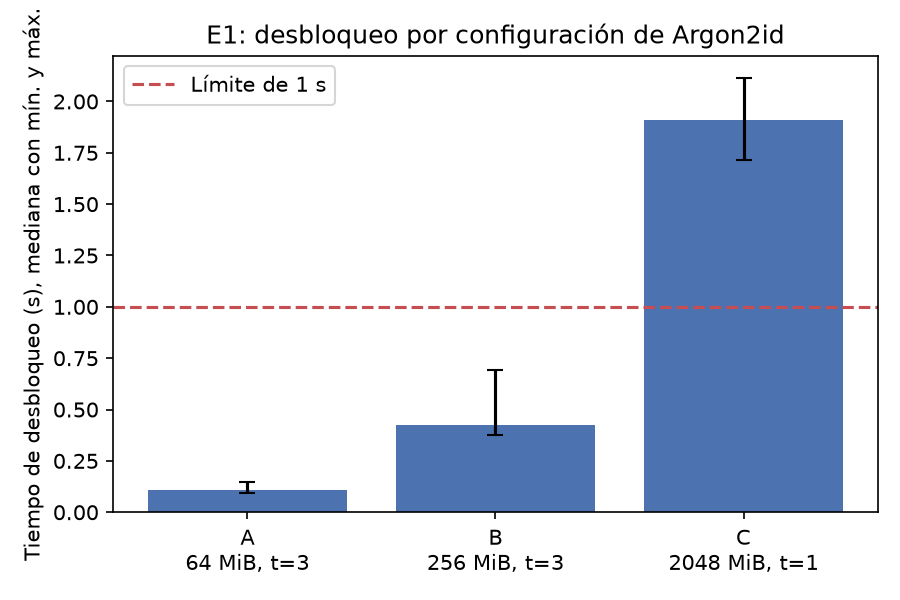
\includegraphics[width=\linewidth]{../../bench/results/e1_desbloqueo.png}
\caption{Desbloqueo por configuración, con el límite de 1 s.}
\end{subfigure}\hfill
\begin{subfigure}{0.49\linewidth}
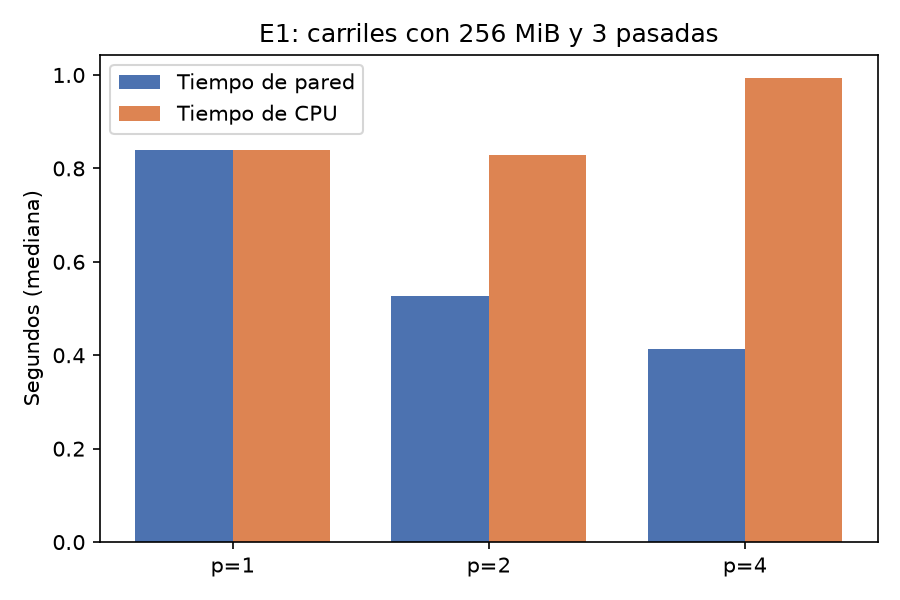
\includegraphics[width=\linewidth]{../../bench/results/e1_carriles.png}
\caption{Tiempo de pared y de CPU según los carriles.}
\end{subfigure}
\caption{Resultados de E1.}
\label{fig:e1}
\end{figure}

\textbf{Carriles.} El Entregable 1 advertía que, si OpenSSL no procesaba los carriles en paralelo, el atacante tendría una ventaja de hasta $p$ veces en tiempo. E1 lo comprobó variando solo $p$ sobre B (figura~\ref{fig:e1}b). Con 1, 2 y 4 carriles el desbloqueo baja de 0,840 a 0,528 y 0,414 s, mientras el tiempo de CPU se mantiene entre 0,83 y 0,99 s, y el cociente entre CPU y pared sube de 1,00 a 1,57 y 2,40. Como \code{process\_time} suma la CPU de todos los hilos, un cociente mayor que 1 prueba que los carriles trabajan a la vez. El defensor aprovecha entonces el paralelismo igual que lo haría un atacante, aunque con 4 carriles la ganancia no llega a 4 veces.

\textbf{Costo de diccionario.} Si un intento cuesta $t$ segundos, recorrer un diccionario $D$ cuesta del orden de $t\cdot|D|$~\cite[§18.4.4]{boneh}. Con B y el $t$ medido, la tabla~\ref{tab:diccionario} da el costo probando un intento a la vez y en horas de núcleo, calculadas con el tiempo de CPU. El $t$ de E1 incluye las comprobaciones 1, 2 y 4, que el atacante podría omitir, pero E2 muestra que pesan unos milisegundos frente a los 422 ms de Argon2id, así que la estimación apenas cambia.

\begin{table}[h]
\centering\small
\caption{Costo estimado de un ataque de diccionario contra la configuración B en el equipo de referencia.}
\label{tab:diccionario}
\begin{tabular}{@{}lrrr@{}}
\toprule
Diccionario & $|D|$ & Un intento a la vez & Horas de núcleo \\
\midrule
Las $10^4$ contraseñas más comunes & $10^4$ & 1,2 h & 2,9 \\
RockYou & $1{,}43\cdot 10^7$ & 1\,683 h (70 días) & 4\,091 \\
Candidatos generados & $10^9$ & 13,4 años & $2{,}9\cdot 10^5$ \\
Contraseña aleatoria de 40 bits & $2^{40}$ & 14\,727 años & $3{,}1\cdot 10^8$ \\
\bottomrule
\end{tabular}
\end{table}

Un intento ocupa unos 2,4 de los 8 hilos del equipo, así que probar en serie no es lo mejor que puede hacer un atacante con él. Si reparte los intentos entre todos los núcleos, y ocho instancias de 256 MiB caben en su memoria, el costo lo dan las horas de núcleo: RockYou le llevaría entre unas 510 h con los 8 hilos y unas 1\,020 h con los 4 núcleos físicos, porque los dos hilos de un núcleo no duplican su rendimiento. Con GPU o muchos núcleos el costo se divide entre los intentos simultáneos, pero cada uno exige 256 MiB de memoria, el recurso escaso del hardware paralelo~\cite{rfc9106}. Una tarjeta con 24 GB, por ejemplo, no sostiene más de unas 90 instancias. Argon2id no vuelve imposible el ataque, lo encarece. Cien equipos como el de referencia recorrerían RockYou en unas 5 a 10 horas, así que una contraseña que esté en un diccionario conocido no queda protegida, y el modelo la deja fuera. En cambio, una contraseña aleatoria de 40 bits les costaría entre unos 45 y 90 años, y cada bit adicional duplica la cifra. La seguridad final depende entonces de la entropía de la contraseña maestra, y Argon2id multiplica el costo de cada candidata por algo más de un segundo de núcleo y 256 MiB de memoria.

\subsection{E2: abrir y guardar sin Argon2id}

E2 usa una KEK aleatoria y mide por separado sellar, la escritura atómica, la lectura con las comprobaciones 1 y 2, y las comprobaciones 3 y 4 con el análisis del JSON, con la mediana de 50 repeticiones (figura~\ref{fig:e2}).

\begin{figure}[h]
\centering
\begin{minipage}{0.49\linewidth}
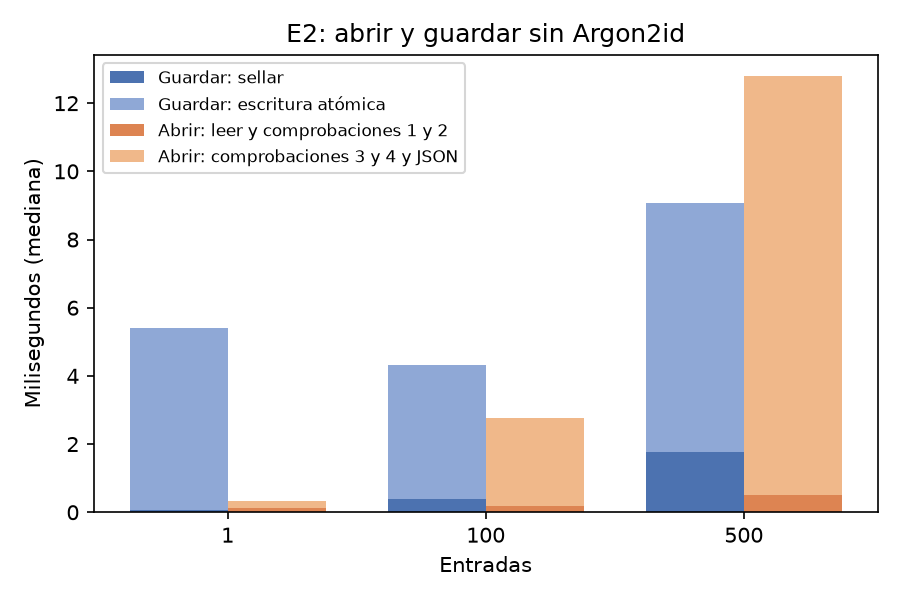
\includegraphics[width=\linewidth]{../../bench/results/e2_abrir_guardar.png}
\end{minipage}\hfill
\begin{minipage}{0.48\linewidth}\small
\begin{tabular}{@{}rrr@{}}
\toprule
Entradas & Guardar & Abrir \\
\midrule
1 & 5,4 ms & 0,4 ms \\
100 & 4,3 ms & 2,8 ms \\
500 & 9,2 ms & 12,8 ms \\
\bottomrule
\end{tabular}
\vspace{1ex}

Guardar lo domina la escritura atómica con sus \code{fsync} (de 3,9 a 7,3 ms) frente a sellar (de 0,07 a 1,8 ms), y la variación de esos \code{fsync} explica que guardar 1 entrada salga más lento que guardar 100. Abrir 500 entradas lo domina el análisis estricto del JSON, no el AEAD.
\end{minipage}
\caption{E2: abrir y guardar con 1, 100 y 500 entradas (mediana de 50).}
\label{fig:e2}
\end{figure}

Frente a los 422 ms del Argon2id de B, abrir y guardar no pesan. Esto valida la decisión de no repetir Argon2id en cada guardado: con la KEK en memoria, cada cambio cuesta milisegundos y cada uno usa una DEK y nonces nuevos.

\subsection{E3: tamaño del archivo}

\begin{figure}[h]
\centering
\begin{minipage}{0.6\linewidth}
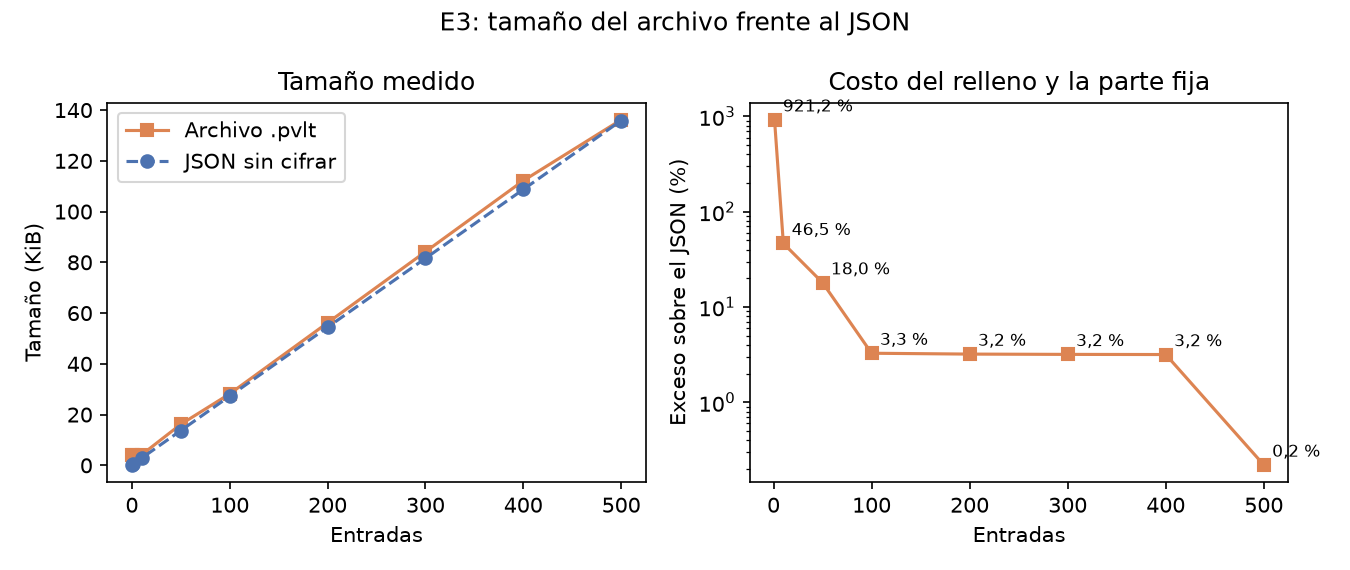
\includegraphics[width=\linewidth]{../../bench/results/e3_tamano.png}
\end{minipage}\hfill
\begin{minipage}{0.37\linewidth}\small
\begin{tabular}{@{}rrr@{}}
\toprule
Entradas & Archivo & Archivo/JSON \\
\midrule
0 & 4\,279 B & 30,1 \\
10 & 4\,279 B & 1,46 \\
100 & 28\,855 B & 1,033 \\
500 & 139\,447 B & 1,002 \\
\bottomrule
\end{tabular}
\end{minipage}
\caption{E3: tamaño del archivo frente al JSON sin cifrar, de 0 a 500 entradas.}
\label{fig:e3}
\end{figure}

El exceso fijo es de 183 bytes y el resto es el JSON más el relleno hasta el siguiente múltiplo de 4096 (figura~\ref{fig:e3}). Por debajo de unas 14 entradas el archivo mide siempre 4\,279 bytes, así que su tamaño no distingue una bóveda vacía de una con una docena de entradas. Desde 100 entradas el archivo ocupa como mucho un 3\,\% más que el JSON. El relleno cumple su función de revelar solo un rango, y su costo es despreciable para bóvedas de este tamaño.

\section{Límites de seguridad y limitaciones}\label{sec:limitaciones}

Cumplir el enunciado no certifica \pvlt{} para uso real. Los resultados anteriores son evidencia dentro del modelo de la sección~\ref{sec:modelo}, y dentro de ese modelo quedan los siguientes límites.

\begin{itemize}
\item \textbf{El SHA-256 final no protege contra manipulación.} Quien altera un campo y recalcula el resumen supera las comprobaciones 1 y 2. Solo sirve para distinguir un fallo de disco de una contraseña incorrecta y ofrecer el respaldo. La integridad la dan las etiquetas AEAD, como muestra T5.
\item \textbf{Mensajes ambiguos por diseño.} Una alteración de la sal, de la cabecera o de $W$ se informa como contraseña incorrecta, porque sin la clave no se puede distinguir.
\item \textbf{Borrado de memoria como esfuerzo razonable.} La KEK se sobrescribe con ceros, pero las bibliotecas guardan copias internas y el contenido descifrado vive en cadenas inmutables de Python y de JavaScript que no pueden borrarse. Por eso los volcados de memoria quedan fuera del modelo.
\item \textbf{Ventana en el cambio de contraseña.} Entre el guardado y la reescritura del respaldo hay un instante en que el \code{.bak} todavía abre con la contraseña anterior. Si el proceso muere justo ahí, el respaldo sigue abriéndose con ella hasta el siguiente guardado.
\item \textbf{Token en los argumentos del navegador.} Fuera de Docker, mientras el sistema lanza el navegador, la URL con el token aparece en los argumentos de ese proceso y un usuario local (A4) podría leerla. Se mitiga porque el token sirve una sola vez: si otro lo canjeara antes, la página del usuario mostraría que el enlace ya se usó.
\item \textbf{Portapapeles.} El borrado a los 20 s no ocurre si se cierra la pestaña antes, y se retrasa hasta que el usuario vuelve a ella si estaba en otra ventana, porque el navegador no deja escribir en el portapapeles sin el foco. También borra lo que el usuario haya copiado entretanto. Es una mitigación parcial, y la interfaz lo advierte.
\item \textbf{Retroceso.} Una copia antigua válida de la bóveda se abre sin error. El contador de generación solo permite advertirlo cuando el respaldo es más reciente, porque no existe un estado externo confiable contra el cual comparar.
\item \textbf{Dependencia del equipo.} La elección de B se hizo en el equipo de referencia. En un equipo más lento B puede superar 1 s, y en uno más rápido convendría una configuración mayor. Para eso \code{python -m bench.calibrate} mide A, B y C en el equipo donde se ejecuta y recomienda con la misma regla la configuración que se elige al crear la bóveda. El formato guarda los parámetros en la cabecera, así que cambiarlos no rompe bóvedas existentes.
\item \textbf{El navegador puede guardar la contraseña maestra.} El campo usa \code{autocomplete="new-password"} y la interfaz recomienda rechazar el guardado, pero algunos navegadores lo ofrecen igual.
\item \textbf{Plataformas.} Las pruebas de fallo y las mediciones se hicieron en Linux dentro de Docker, con la semántica POSIX de \code{fsync} y \code{os.replace}. Windows y macOS se consideran compatibles, pero no se evaluaron como plataformas de referencia.
\end{itemize}

\section{Conclusiones}

\pvlt{} implementa el diseño del Entregable 1 sin desviaciones de formato ni de protocolo. La jerarquía KEK y DEK con una DEK nueva por guardado resolvió la unicidad de nonces sin contadores persistentes, y la cabecera como dato asociado con etiquetas de dominio hizo que cualquier alteración del archivo se rechace, como verifican las pruebas de manipulación sobre cada campo. Validar los parámetros antes de Argon2id y separar las cuatro comprobaciones permitió dar a cada fallo un mensaje propio sin escribir nunca en disco. El guardado atómico con respaldo resistió una caída tras cada uno de sus pasos.

Los experimentos confirmaron los supuestos que el diseño dejó abiertos. Los carriles de Argon2id corren en paralelo, el pico de memoria coincide con el parámetro elegido y la configuración B, de 256 MiB, desbloquea en 0,42 s mientras impone a un atacante unas 4\,100 horas de núcleo, entre tres y seis semanas de este mismo equipo a pleno uso, por cada diccionario del tamaño de RockYou. Abrir y guardar cuestan milisegundos frente a ese costo, y el relleno solo deja ver un rango del tamaño de la bóveda.

Las limitaciones que quedan son las propias de una aplicación local escrita en un lenguaje con memoria administrada, más algunas ventanas pequeñas y documentadas. Ninguna contradice el modelo de adversario propuesto. Como trabajo futuro quedan medir en hardware paralelo el costo real de un atacante con GPU, integrar en la creación de la bóveda la calibración de Argon2id que hoy se ejecuta aparte y evaluar Windows y macOS como plataformas de referencia.

\begin{thebibliography}{9}\small
\setlength{\itemsep}{1pt}
\bibitem{boneh} Boneh, D. y Shoup, V. (2023). \emph{A Graduate Course in Applied Cryptography}, v0.6, §§9.5 y 18.4.4.
\bibitem{rfc9106} Biryukov, A., Dinu, D., Khovratovich, D. y Josefsson, S. (2021). \emph{Argon2 Memory-Hard Function for Password Hashing and Proof-of-Work Applications}. RFC 9106.
\bibitem{rfc8439} Nir, Y. y Langley, A. (2018). \emph{ChaCha20 and Poly1305 for IETF Protocols}. RFC 8439.
\bibitem{sp80038d} Dworkin, M. (2007). \emph{Recommendation for Block Cipher Modes of Operation: Galois/Counter Mode (GCM) and GMAC}. NIST SP 800-38D.
\bibitem{protocols} Villanueva-Polanco, R. \emph{Cryptographic Protocols} (Protocols.pdf), material del curso, diapositivas 17 a 43 y 193 a 195.
\bibitem{enunciado} Villanueva-Polanco, R. \emph{Banco de Proyectos I+D en Criptografía Aplicada}, Proyecto 2.
\bibitem{owasp} OWASP. \emph{Cross-Site Request Forgery Prevention Cheat Sheet}. OWASP Cheat Sheet Series. \url{https://cheatsheetseries.owasp.org}
\bibitem{pyca} Python Cryptographic Authority. \emph{cryptography} 50.0.2, documentación de \code{Argon2id} y \code{ChaCha20Poly1305}. \url{https://cryptography.io}
\end{thebibliography}

\end{document}
